\documentclass{article}

\usepackage[left=1in, right=1in, top=1.2in, bottom=1.2in]{geometry}
\usepackage{graphicx}
\usepackage{amsmath}
\usepackage{amssymb}
\usepackage{amsthm}
\usepackage{mathtools}
\usepackage[most]{tcolorbox}
\usepackage{bbm}
\usepackage{hyperref}
\usepackage{booktabs}
\usepackage[title]{appendix}
\usepackage{enumitem}
\usepackage{algorithm}
\usepackage{algorithmic}

\newcommand{\loss}{\mathcal{L}}
\newcommand{\Id}{\mathbbm{1}}
\newcommand{\vecb}[1]{\boldsymbol{#1}}

\title{Induced Metric Optimisers}
\date{\today}

\begin{document}

\maketitle
\tableofcontents
\newpage


%%%%%%%%%%%%%%%%%%%%%%%%%%%%%%%%%%%%%%%%%%%%%%%%%%%%%%%%%%%%%
%%%%%%%%%%%%%%%%%%%%%%%%%%%%%%%%%%%%%%%%%%%%%%%%%%%%%%%%%%%%%
\section{Introduction}\label{sec:intro}
%%%%%%%%%%%%%%%%%%%%%%%%%%%%%%%%%%%%%%%%%%%%%%%%%%%%%%%%%%%%%
%%%%%%%%%%%%%%%%%%%%%%%%%%%%%%%%%%%%%%%%%%%%%%%%%%%%%%%%%%%%%

Harvey~\cite{harvey2025} introduced a class of optimisers that precondition gradients
using the Riemannian metric naturally induced when the loss landscape is embedded in
higher-dimensional space.
The key idea is to embed the $N$-dimensional parameter space into $\mathbb{R}^{N+1}$
via the loss function, equip the ambient space with a metric~$h$, and pull~$h$ back to
obtain a geometry-aware preconditioner.
The resulting update automatically damps the effective learning rate in high-curvature
regions---acting as a smooth form of gradient clipping---while adding only $O(N)$ overhead.

This document extends that framework in three directions
(summarised in Table~\ref{tab:variants}):

\begin{enumerate}[label=(\roman*)]
    \item \textbf{Learnable scalar metric} (Section~\ref{sec:scalar}):
    the inverse base metric $\gamma^{-1}$ is parameterised by a single learnable scalar $s$,
    allowing the overall metric scale to adapt during training.

    \item \textbf{Learnable diagonal metric} (Section~\ref{sec:diag}):
    each parameter receives its own learnable scale $s_i$,
    enabling per-parameter metric adaptation with a principled
    gauge-fixing (mean-centering) to remove the degeneracy with the global
    scaling hyperparameter~$\xi$.

    \item \textbf{Off-diagonal ambient metric} (Section~\ref{sec:offdiag}):
    the ambient metric $h$ in~\cite{harvey2025} has no coupling between
    the parameter dimensions and the loss dimension (the off-diagonal blocks are zero).
    We relax this by introducing coupling vectors $\vecb{a}$ and $\vecb{b}$,
    which add a second component to the update direction
    and enable geometry-induced momentum, weight decay, and other behaviours.
\end{enumerate}

\begin{table}[ht]
\centering
\caption{Summary of optimiser variants.
All share the same geometric construction (embed, pull back, invert via Sherman-Morrison-Woodbury)
and are $O(N)$ per step.
Sections~\ref{sec:scalar}--\ref{sec:offdiag} are the new contributions of this document.}
\label{tab:variants}
\small
\begin{tabular}{@{}llcc@{}}
    \toprule
    \textbf{Variant} & \textbf{Base metric $\gamma^{ij}$} & \textbf{Learnable?} & \textbf{Section} \\
    \midrule
    Fixed diagonal     & $\gamma\,\delta^{ij}$ (hyperparameter)     & No  & \ref{sec:fixed} \\
    Learnable scalar   & $e^s\,\delta^{ij}$                         & Yes ($s\in\mathbb{R}$) & \ref{sec:scalar} \\
    Learnable diagonal & $e^{s_i}\,\delta^{ij}$                     & Yes ($\vecb{s}\in\mathbb{R}^N$) & \ref{sec:diag} \\
    Off-diagonal       & $\gamma\,\delta^{ij}$ + off-diag.\ $\vecb{a},\vecb{b}$ & No & \ref{sec:offdiag} \\
    \bottomrule
\end{tabular}
\end{table}

\noindent
\textbf{Roadmap.}\quad
Section~\ref{sec:setup} establishes notation.
Section~\ref{sec:fixed} reproduces the core method of~\cite{harvey2025},
including the full algorithms, and defines the practical machinery
(momentum, EMA, log-loss variant) used by all subsequent sections.
The three extensions follow in Sections~\ref{sec:scalar}--\ref{sec:offdiag},
each with its own algorithm.
Section~\ref{sec:shared} collects implementation details common to all variants,
and Section~\ref{sec:results} presents benchmark results.
Appendix~\ref{app:repo} documents the repository structure and sweep infrastructure.

\paragraph{A note on what is being learned.}
In the learnable variants (Sections~\ref{sec:scalar} and~\ref{sec:diag}),
we parameterise and learn the \emph{inverse} base metric $\gamma^{ij}$,
not the metric $\gamma_{ij}$ itself.
This is natural because the update rule requires $\gamma^{-1}$,
and parameterising the inverse directly avoids an inversion step.


%%%%%%%%%%%%%%%%%%%%%%%%%%%%%%%%%%%%%%%%%%%%%%%%%%%%%%%%%%%%%
%%%%%%%%%%%%%%%%%%%%%%%%%%%%%%%%%%%%%%%%%%%%%%%%%%%%%%%%%%%%%
\section{Setup and Notation}\label{sec:setup}
%%%%%%%%%%%%%%%%%%%%%%%%%%%%%%%%%%%%%%%%%%%%%%%%%%%%%%%%%%%%%
%%%%%%%%%%%%%%%%%%%%%%%%%%%%%%%%%%%%%%%%%%%%%%%%%%%%%%%%%%%%%
Given a model with $N$ parameters $\theta(t)=\{\theta^i(t)\}_{i=1}^N$ and a loss function
$\loss:\mathbb{R}^N\to\mathbb{R}$,
our goal is to find the optimal parameter update $\delta \theta$ at each time step $t$.
That is, in preconditioned gradient flow we have $$
    \frac{d \theta^i}{dt} = - g^{ij} \frac{\partial \loss}{\partial \theta^j}
    \implies
    \delta \theta^i \approx - \eta g^{ij} \frac{\partial \loss}{\partial \theta^j}
$$ where $\eta\in\mathbb{R}_{>0}$ is the learning rate and $g^{ij}$ is the inverse of the induced metric on the parameter space.

Across all variants in this document the induced metric is obtained by the same geometric construction:
we embed parameter space into an ambient space via $$
    \phi:\mathbb{R}^N\to\mathbb{R}^{N+1}, \qquad
    \phi(\theta^1,\ldots,\theta^N) = (\theta^1,\ldots,\theta^N,f(\theta)),
$$ where $f:\mathbb{R}^N\to\mathbb{R}$ is a scalar function of the parameters (taken to be the loss $\loss$, or a function thereof), and then pull back an ambient bilinear form $h\in\mathbb{R}^{(N+1)\times(N+1)}$ to the parameter space.
The variants differ in the choice of $h$ (and, for the log-loss variant, the embedding function $f$; see below).

We use the shorthand $l_i\coloneqq \partial \loss/\partial\theta^i$ for the raw gradient.
When a base metric $\gamma_{ij}$ is present, we write $l^i \coloneqq \gamma^{ij} l_j$ for the
metric-raised gradient (i.e.\ the inverse metric applied to $\vecb{l}$).
When $\gamma = \Id_N$ (the identity), raising an index has no effect, so $l^i = l_i$ and the two notations coincide.
The same index-raising convention applies to any covector:
$a^i \coloneqq \gamma^{ij}a_j$, $m^i \coloneqq \gamma^{ij}m_j$, etc.


%%%%%%%%%%%%%%%%%%%%%%%%%%%%%%%%%%%%%%%%%%%%%%%%%%%%%%%%%%%%%
%%%%%%%%%%%%%%%%%%%%%%%%%%%%%%%%%%%%%%%%%%%%%%%%%%%%%%%%%%%%%
\section{Fixed Diagonal Metric}\label{sec:fixed}
%%%%%%%%%%%%%%%%%%%%%%%%%%%%%%%%%%%%%%%%%%%%%%%%%%%%%%%%%%%%%
%%%%%%%%%%%%%%%%%%%%%%%%%%%%%%%%%%%%%%%%%%%%%%%%%%%%%%%%%%%%%
This section reproduces the core method of \cite{harvey2025}:
a fixed base metric $\gamma$ defines the ambient space geometry,
and the induced metric on parameter space provides a preconditioner
for gradient descent.
The geometric derivation, practical algorithms,
and all notation established here
carry forward to the extensions in
Sections~\ref{sec:scalar}--\ref{sec:offdiag}.

\subsection{Geometric Derivation}

The original ambient metric in \cite{harvey2025} is $$
    h = \begin{pmatrix} \gamma & \vecb{0} \\ \vecb{0}^\top & 1 \end{pmatrix}\in\mathbb{R}^{(N+1)\times(N+1)}
$$ where $\gamma\in\mathbb{R}^{N\times N}$ is symmetric positive-definite (taken to be diagonal or scalar in all our experiments).
The induced metric $g$ on the parameter space is given by $$
    g_{ij}
    = h_{\alpha\beta} \frac{\partial \phi^\alpha}{\partial \theta^i} \frac{\partial \phi^\beta}{\partial \theta^j}
    = \gamma_{ij} + \frac{\partial \loss}{\partial \theta^i} \frac{\partial \loss}{\partial \theta^j}.
$$ Then, to calculate the parameter updates $\delta \theta^i$ we need $g^{ij}$, the inverse of $g_{ij}$.
We can compute this inverse using the Sherman-Morrison-Woodbury formula:
\begin{tcolorbox}[colback=gray!8, colframe=gray!22, breakable, title=\textbf{Sherman-Morrison-Woodbury Formula}, coltitle=black]
    Let $A\in\mathbb{R}^{n\times n}$ be an invertible matrix, and let $U,V\in\mathbb{R}^{n\times k}$ be matrices.
    Then, if $C = A + U V^\top$ is invertible, we have $$C^{-1} = A^{-1} - A^{-1} U (I_k + V^\top A^{-1} U)^{-1} V^\top A^{-1}.$$
\end{tcolorbox}
\noindent This gives us $$
    g^{ij}
    = \gamma^{ij} - \frac{\gamma^{ik}\gamma^{jl} \frac{\partial \loss}{\partial \theta^k} \frac{\partial \loss}{\partial \theta^l}}{1 + \gamma^{mn} \frac{\partial \loss}{\partial \theta^m} \frac{\partial \loss}{\partial \theta^n}}
    = \gamma^{ij} - \frac{l^i l^j}{1+l_k l^k}
$$ where $$
    l_i \coloneqq \frac{\partial\loss}{\partial \theta^i} \implies l^i = \gamma^{ij} l_j.
$$ Thus, the parameter updates are given by
\begin{align*}
    \delta \theta^i =& -\eta \left( \gamma^{ij} - \frac{l^i l^j}{1+l_k l^k} \right) l_j \\
    =& -\eta l^i \left( 1 - \frac{l_j l^j}{1+l_k l^k} \right) \\
    =& -\eta l^i \left( \frac{1}{1+l_k l^k} \right).
\end{align*}

So to summarize, (1) we start with an ambient metric $h$ which induces a metric $g$ on the parameter space,
(2) we compute the inverse $g^{ij}$, and
(3) we use $g^{ij}$ to compute the parameter updates $\delta \theta^i$.

\subsection{Practical Algorithm}\label{sec:practical}

The theoretical update above becomes a practical optimiser by adding
a hyperparameter $\xi$ to control the metric strength,
momentum with bias correction,
an exponential moving average (EMA) for the denominator,
and decoupled weight decay.
The full procedure is given in Algorithm~\ref{alg:fixed}
(adapted from Algorithm~1 of~\cite{harvey2025}).
The log-loss variant is Algorithm~\ref{alg:fixed-log}
(adapted from Algorithm~2 of~\cite{harvey2025}).

\begin{algorithm}[H]
\caption{Fixed diagonal metric (plain embedding, $f=\loss$)}
\label{alg:fixed}
\begin{algorithmic}[1]
\REQUIRE learning rate $\eta$, momentum decay $\beta_m$, metric strength $\xi$, denominator EMA decay $\beta$, weight decay $\lambda_\theta$, inverse base metric $\gamma^{-1}$
\STATE Initialise $t \leftarrow 0$, $\vecb{m}_0 \leftarrow \vecb{0}$, $\bar{v}_0 \leftarrow 0$
\WHILE{$\theta_t$ not converged}
\STATE $t \leftarrow t + 1$
\STATE $\vecb{l}_t \leftarrow \nabla_\theta \loss(\theta_{t-1})$
\STATE $v_t \leftarrow \xi \cdot \sum_i l_{t,i}\,(\gamma^{-1}\vecb{l}_t)_i$
    \hfill{\footnotesize\textit{// trace statistic}}
\STATE $\bar{v}_t \leftarrow \beta\,\bar{v}_{t-1} + (1-\beta)\,v_t$
    \hfill{\footnotesize\textit{// denominator EMA}}
\STATE $\hat{v}_t \leftarrow \bar{v}_t / (1 - \beta^t)$
    \hfill{\footnotesize\textit{// bias correction}}
\STATE $r_t \leftarrow 1/(1 + |\hat{v}_t|)$
    \hfill{\footnotesize\textit{// damping factor}}
\STATE $\vecb{m}_t \leftarrow \beta_m\,\vecb{m}_{t-1} + (1-\beta_m)\,\vecb{l}_t$
    \hfill{\footnotesize\textit{// momentum}}
\STATE $\hat{\vecb{m}}_t \leftarrow \gamma^{-1}\vecb{m}_t / (1 - \beta_m^t)$
    \hfill{\footnotesize\textit{// bias-corrected, metric-raised}}
\STATE $\theta_t \leftarrow \theta_{t-1} - \eta\,r_t\,\hat{\vecb{m}}_t - \eta\,\lambda_\theta\,\theta_{t-1}$
\ENDWHILE
\RETURN $\theta_t$
\end{algorithmic}
\end{algorithm}

\begin{algorithm}[H]
\caption{Fixed diagonal metric (log-loss embedding, $f=\log\loss$, requires $\loss>0$)}
\label{alg:fixed-log}
\begin{algorithmic}[1]
\REQUIRE same as Algorithm~\ref{alg:fixed}
\STATE Initialise $t \leftarrow 0$, $\vecb{m}_0 \leftarrow \vecb{0}$, $\bar{v}_0 \leftarrow 0$
\WHILE{$\theta_t$ not converged}
\STATE $t \leftarrow t + 1$
\STATE $\vecb{l}_t \leftarrow \nabla_\theta \loss(\theta_{t-1})$;\quad $L_t \leftarrow \loss(\theta_{t-1})$
\STATE $v_t \leftarrow \xi \cdot \sum_i l_{t,i}\,(\gamma^{-1}\vecb{l}_t)_i$
\STATE $\bar{v}_t \leftarrow \beta\,\bar{v}_{t-1} + (1-\beta)\,v_t$;\quad $\hat{v}_t \leftarrow \bar{v}_t / (1 - \beta^t)$
\STATE $r_t \leftarrow L_t / (L_t^2 + |\hat{v}_t|)$
    \hfill{\footnotesize\textit{// log-loss damping}}
\STATE $\vecb{m}_t \leftarrow \beta_m\,\vecb{m}_{t-1} + (1-\beta_m)\,\vecb{l}_t$;\quad $\hat{\vecb{m}}_t \leftarrow \gamma^{-1}\vecb{m}_t / (1 - \beta_m^t)$
\STATE $\theta_t \leftarrow \theta_{t-1} - \eta\,r_t\,\hat{\vecb{m}}_t - \eta\,\lambda_\theta\,\theta_{t-1}$
\ENDWHILE
\RETURN $\theta_t$
\end{algorithmic}
\end{algorithm}

\noindent
In short, the practical update at each step is
\begin{equation}\label{eq:fixed-update}
    \delta\theta^i = -\eta\,r_t\,\hat{m}^i, \qquad
    r_t = \frac{1}{1 + |\hat{v}_t|}, \qquad
    v_t = \xi\,\gamma^{mn}\,l_{t,m}\,l_{t,n},
\end{equation}
where $\hat{v}_t$ is the bias-corrected EMA of $v_t$
(lines~6--8 of Algorithm~\ref{alg:fixed})
and $\hat{m}^i$ is the bias-corrected, metric-raised momentum (line~10).

\subsection{Log-Loss Variant}

\begin{tcolorbox}[colback=gray!8, colframe=gray!22, breakable, title=\textbf{Log-Loss Derivation Sketch}, coltitle=black]
    With $f = \log\loss$ the embedding gradient is $\partial f/\partial\theta^i = l_i/\loss$,
    so the induced metric becomes
    $g_{ij} = \gamma_{ij} + \xi\,(l_i/\loss)(l_j/\loss)$.
    Applying Sherman-Morrison-Woodbury gives the inverse metric
    $$
        g^{ij} = \gamma^{ij} - \frac{\xi\,l^i l^j}{\loss^2 + \xi\,l_k l^k}.
    $$
    Contracting with the \emph{raw} gradient $l_j$ yields
    $g^{ij}l_j = l^i \cdot \loss^2/(\loss^2 + v_t)$,
    where $v_t = \xi\,\gamma^{mn}\,l_m\,l_n$.

    \medskip\noindent
    The full geometric update, however, uses the embedding gradient
    $\partial_j f = l_j/\loss$, not the raw gradient:
    $$
        g^{ij}\frac{\partial f}{\partial\theta^j}
        = \frac{g^{ij}l_j}{\loss}
        = l^i \cdot \frac{\loss}{\loss^2 + v_t}.
    $$
    The practical damping factor $r_t = \loss_t/(\loss_t^2 + |\hat{v}_t|)$
    (line~7 of Algorithm~\ref{alg:fixed-log})
    therefore follows directly from the geometry of the log embedding.
    This provides stronger damping than $\loss^2/(\loss^2 + |\hat{v}_t|)$
    as $\loss\to 0$, preventing overshooting near minima.
\end{tcolorbox}

\noindent In practice, the update direction $\vecb{u}$ and the metric direction $\vecb{l}$
need not coincide; see Section~\ref{sec:shared} for the full treatment.

\subsection{Implementation}
\begin{itemize}
    \item JAX/Optax: \href{https://github.com/Noah-Everett/Induced-Metric-Optimiser/blob/main/optimisers/jax_fixed.py}{\texttt{optimisers/jax\_fixed.py}}
    \item PyTorch: \href{https://github.com/Noah-Everett/Induced-Metric-Optimiser/blob/main/optimisers/torch_fixed.py}{\texttt{optimisers/torch\_fixed.py}}
    \item Equivalence check: \href{https://github.com/Noah-Everett/Induced-Metric-Optimiser/blob/main/optimisers/compare_fixed.py}{\texttt{optimisers/compare\_fixed.py}}
\end{itemize}
\begin{sloppypar}
Exposed optimisers: \texttt{custom\_sgd} (plain embedding, $f=\loss$),
\texttt{custom\_sgd\_log} (log-loss embedding, $f=\log\loss$; requires $\loss>0$),
\texttt{custom\_sgd\_rms} (RMS-normalised gradients, i.e.\ the update direction is
$l_i/\|\vecb{l}\|$ instead of $l_i$).
The sweep name is \texttt{sgd\_metric} / \texttt{sgd\_log\_metric} / \texttt{sgd\_rms}.
\end{sloppypar}


%%%%%%%%%%%%%%%%%%%%%%%%%%%%%%%%%%%%%%%%%%%%%%%%%%%%%%%%%%%%%
%%%%%%%%%%%%%%%%%%%%%%%%%%%%%%%%%%%%%%%%%%%%%%%%%%%%%%%%%%%%%
\section{Learnable Scalar Metric}\label{sec:scalar}
%%%%%%%%%%%%%%%%%%%%%%%%%%%%%%%%%%%%%%%%%%%%%%%%%%%%%%%%%%%%%
%%%%%%%%%%%%%%%%%%%%%%%%%%%%%%%%%%%%%%%%%%%%%%%%%%%%%%%%%%%%%

The fixed diagonal variant treats $\gamma$ as a hyperparameter chosen before training.
A natural next step is to let the metric adapt during optimisation.
We begin with the simplest case: a single learnable scalar
that controls the global scale of $\gamma^{-1}$.

\subsection{Construction}
We parameterise the inverse metric as $$
    \gamma^{ij} = \alpha\,\delta^{ij}, \qquad \alpha = e^s,
$$ where $s\in\mathbb{R}$ is a single learnable scalar.
(We learn the \emph{inverse} metric directly because the update rule requires $\gamma^{-1}$.)
Initialising $s=0$ gives $\gamma^{-1}=\Id_N$, so the optimiser starts as the unscaled fixed diagonal variant.

The ambient metric remains block-diagonal, $$
    h = \begin{pmatrix} e^{-s}\,\Id_N & \vecb{0} \\ \vecb{0}^\top & 1 \end{pmatrix},
$$ and the induced metric on parameter space is $$
    g_{ij} = e^{-s}\,\delta_{ij} + l_i l_j.
$$
Applying the Sherman-Morrison-Woodbury formula with $A_{ij}=e^{-s}\delta_{ij}$, $u=v=\vecb{l}$:
$$
    g^{ij} = e^s\,\delta^{ij} - \frac{l^i\,l^j}{1 + l_k l^k}.
$$
Here $l^i = \gamma^{ij}l_j = e^s l_i$,
so $l^i l^j = e^{2s} l_i l_j$ and $l_k l^k = e^s\|\vecb{l}\|^2$.
The parameter update is therefore
\begin{align*}
    \delta\theta^i
    &= -\eta\,g^{ij}l_j
    = -\eta\,l^i\left(1 - \frac{l_j l^j}{1+l_k l^k}\right)
    = -\frac{\eta\,l^i}{1 + l_k l^k}.
\end{align*}
Since $l_k l^k = e^s\|\vecb{l}\|^2$, the denominator depends on $s$ through the metric.
The practical update follows the same structure as \eqref{eq:fixed-update},
with $\gamma^{ij} = \alpha\,\delta^{ij}$ and the trace statistic specialised to
\begin{equation}\label{eq:scalar-update}
    v_t = \xi\,\alpha\,\|\vecb{l}_t\|^2.
\end{equation}

\subsection{Metric Learning}\label{sec:scalar-learning}
We want to learn $s$ so that $\alpha = e^s$ is calibrated to the local geometry of the loss.
The trace statistic $v_t = \xi\alpha\|\vecb{l}_t\|^2$ is the quantity that controls
the denominator damping in the update rule:
it measures how strongly the gradient stretches the embedded loss surface
under the current metric.
The only scalar that couples $\gamma$ to the gradient $\vecb{l}$ is $v_t$ itself,
making it the natural surrogate objective for adapting~$s$.

We perform \emph{gradient ascent} on $v_t$ with respect to $s$:
$$
    \frac{\partial v_t}{\partial s} = \xi\,e^s\,\|\vecb{l}_t\|^2 = v_t.
$$

\paragraph{Why ascent?}
Increasing $s$ increases $\alpha = e^s$, which amplifies
the preconditioned direction $\alpha\hat{\vecb{m}}$ in the numerator.
At the same time, $v_t$ (and hence $\hat{v}_t$) grows,
which shrinks the damping factor $r_t = 1/(1+|\hat{v}_t|)$ in the denominator.
These two effects partially cancel: the metric becomes more responsive
to the gradient structure, but the self-regulating denominator prevents
the step size from blowing up.
Gradient \emph{descent} on $v_t$ would push $s \to -\infty$,
collapsing the metric towards zero and making the optimiser ignore the geometry entirely.
Ascent keeps the metric ``engaged'' with the loss landscape.

\paragraph{Regularisation and stability.}
Note that $v_t\ge 0$, so the unregularised ascent rule monotonically increases~$s$.
Left unchecked this would eventually saturate the clipping bound.
Three mechanisms prevent this:
(i)~an L2 regularisation term $-\mu\lambda s$ that provides a restoring force towards $s=0$ (i.e.\ $\gamma^{-1}=\Id$),
(ii)~hard clipping of $s$ to $[-s_{\max}, s_{\max}]$, and
(iii)~the denominator EMA itself, which smooths transient gradient spikes.
The resulting dynamics should be viewed as a stabilised feedback controller rather
than an unbiased estimator of an optimal metric parameter.

The online metric update is
\begin{equation}\label{eq:scalar-meta}
    s \;\leftarrow\; s + \mu\,v_t - \mu\,\lambda\,s,
\end{equation}
where $\mu>0$ is the metric learning rate and $\lambda>0$ is the L2 regularisation coefficient,
followed by clipping to $[-s_{\max}, s_{\max}]$.

\subsection{Algorithm}

\begin{algorithm}[H]
\caption{Learnable scalar metric (plain embedding)}
\label{alg:scalar}
\begin{algorithmic}[1]
\REQUIRE all hyperparameters from Algorithm~\ref{alg:fixed},
plus metric learning rate $\mu$, metric regularisation $\lambda$, clipping bound $s_{\max}$
\STATE Initialise $t \leftarrow 0$, $\vecb{m}_0 \leftarrow \vecb{0}$, $\bar{v}_0 \leftarrow 0$, $s \leftarrow 0$
\WHILE{$\theta_t$ not converged}
\STATE $t \leftarrow t + 1$;\quad $\alpha \leftarrow e^s$
\STATE $\vecb{l}_t \leftarrow \nabla_\theta \loss(\theta_{t-1})$
\STATE $v_t \leftarrow \xi\,\alpha\,\|\vecb{l}_t\|^2$
\STATE $\bar{v}_t \leftarrow \beta\,\bar{v}_{t-1} + (1-\beta)\,v_t$;\quad
  $\hat{v}_t \leftarrow \bar{v}_t / (1-\beta^t)$;\quad
  $r_t \leftarrow 1/(1+|\hat{v}_t|)$
\STATE $\vecb{m}_t \leftarrow \beta_m\,\vecb{m}_{t-1} + (1-\beta_m)\,\vecb{l}_t$;\quad
  $\hat{\vecb{m}}_t \leftarrow \alpha\,\vecb{m}_t/(1-\beta_m^t)$
\STATE $\theta_t \leftarrow \theta_{t-1} - \eta\,r_t\,\hat{\vecb{m}}_t - \eta\,\lambda_\theta\,\theta_{t-1}$
    \hfill{\footnotesize\textit{// parameter update}}
\STATE $s \leftarrow s + \mu\,v_t - \mu\,\lambda\,s$
    \hfill{\footnotesize\textit{// metric update}}
\STATE $s \leftarrow \operatorname{clip}(s,\,-s_{\max},\,s_{\max})$
\ENDWHILE
\RETURN $\theta_t$
\end{algorithmic}
\end{algorithm}

\noindent
The log-loss variant replaces line~6 with
$r_t \leftarrow L_t/(L_t^2 + |\hat{v}_t|)$.

\subsection{Hyperparameters}
The learnable scalar variant introduces three new hyperparameters beyond those of the fixed diagonal variant:
\begin{itemize}
    \item $\mu$ (\texttt{metric\_lr}): step size for the online metric update in \eqref{eq:scalar-meta}.
    \item $\lambda$ (\texttt{metric\_reg}): L2 regularisation strength on $s$, controlling how far the metric drifts from identity.
    \item $s_{\max}$ (\texttt{metric\_clip}): clipping bound on $s$, bounding $\alpha\in[e^{-s_{\max}}, e^{s_{\max}}]$.
\end{itemize}

\subsection{Implementation}
\begin{itemize}
    \item JAX/Optax: \href{https://github.com/Noah-Everett/Induced-Metric-Optimiser/blob/main/optimisers/jax_learnable_scalar.py}{\texttt{optimisers/jax\_learnable\_scalar.py}}
    \item PyTorch: \href{https://github.com/Noah-Everett/Induced-Metric-Optimiser/blob/main/optimisers/torch_learnable_scalar.py}{\texttt{optimisers/torch\_learnable\_scalar.py}}
    \item Equivalence check: \href{https://github.com/Noah-Everett/Induced-Metric-Optimiser/blob/main/optimisers/compare_learnable_scalar.py}{\texttt{optimisers/compare\_learnable\_scalar.py}}
\end{itemize}
\begin{sloppypar}
The plain variant is \texttt{custom\_sgd\_learnable\_scalar} (sweep: \texttt{sgd\_learn\_scalar}).
The log-loss variant is \texttt{custom\_sgd\_log\_learnable\_scalar} (sweep: \texttt{sgd\_learn\_scalar\_log}).
\end{sloppypar}


%%%%%%%%%%%%%%%%%%%%%%%%%%%%%%%%%%%%%%%%%%%%%%%%%%%%%%%%%%%%%
%%%%%%%%%%%%%%%%%%%%%%%%%%%%%%%%%%%%%%%%%%%%%%%%%%%%%%%%%%%%%
\section{Learnable Diagonal Metric}\label{sec:diag}
%%%%%%%%%%%%%%%%%%%%%%%%%%%%%%%%%%%%%%%%%%%%%%%%%%%%%%%%%%%%%
%%%%%%%%%%%%%%%%%%%%%%%%%%%%%%%%%%%%%%%%%%%%%%%%%%%%%%%%%%%%%

The learnable scalar metric has a single degree of freedom and therefore applies
the same scale to every parameter.
We now generalise to a per-parameter learnable scale,
giving each parameter its own adaptive metric entry.

\subsection{Construction}
We promote $s$ to a full vector $\vecb{s}\in\mathbb{R}^N$ with one entry per parameter,
giving the per-parameter inverse metric $$
    \gamma^{ij} = e^{s_i}\,\delta^{ij}.
$$
The ambient metric is $$
    h = \begin{pmatrix} \operatorname{diag}(e^{-\vecb{s}}) & \vecb{0} \\ \vecb{0}^\top & 1 \end{pmatrix},
$$ and the induced metric on parameter space is $$
    g_{ij} = e^{-s_i}\,\delta_{ij} + l_i l_j.
$$
This is again a rank-1 update to a diagonal matrix.
Applying Sherman-Morrison-Woodbury with $A_{ij} = e^{-s_i}\delta_{ij}$ and $u=v=\vecb{l}$,
$$
    g^{ij} = e^{s_i}\,\delta^{ij} - \frac{l^i\,l^j}{1 + l_k l^k},
$$
where $l^i = \gamma^{ij}l_j = e^{s_i}l_i$ (no sum on $i$),
so $l^i l^j = e^{s_i}l_i\cdot e^{s_j}l_j$ and $l_k l^k = \sum_k e^{s_k}l_k^2$.
The update is
\begin{align*}
    \delta\theta^i
    &= -\eta\,g^{ij}l_j
    = -\eta\left(l^i - \frac{l^i\,(l_k l^k)}{1+l_k l^k}\right)
    = -\frac{\eta\,l^i}{1+l_k l^k}.
\end{align*}
With $\xi$, momentum, and the EMA damping, the practical update is
\begin{equation}\label{eq:diag-update}
    \delta\theta^i = -\eta\,r_t\,\hat{m}^i, \qquad
    r_t = \frac{1}{1 + |\hat{v}_t|}, \qquad
    v_t = \xi\sum_k e^{s_k}\,l_k^2,
\end{equation}
with the same log-loss variant as before.
Compared to the scalar case, each parameter $\theta^i$ now has an individual scale $e^{s_i}$,
allowing the metric to adapt separately to different regions of parameter space.

\subsection{Metric Learning}
The per-parameter metric update treats each $s_i$ independently.
We use the same surrogate-ascent strategy as in Section~\ref{sec:scalar-learning},
now applied to the trace statistic $v_t = \xi\sum_k e^{s_k}l_k^2$
which serves as the surrogate objective:
$$
    J(\vecb{s}) = v_t = \xi\sum_k e^{s_k}\,l_k^2.
$$
This is the natural choice: $v_t$ is the scalar that appears in the denominator of the update rule
and it is the only quantity that couples all of $\gamma$, $\vecb{l}$, and $\vecb{s}$.
Its gradient with respect to $s_i$ is $$
    \frac{\partial J}{\partial s_i} = \xi\,e^{s_i}\,l_i^2.
$$
The online update is therefore
\begin{equation}\label{eq:diag-meta}
    s_i \;\leftarrow\; s_i + \mu\,\xi\,e^{s_i}\,l_i^2 - \mu\,\lambda\,s_i,
\end{equation}
followed by mean-centering and clipping (discussed below).
The motivation for gradient \emph{ascent} (not descent) and the role of regularisation
are the same as in Section~\ref{sec:scalar-learning}.

\subsection{Mean-Centering}\label{sec:mean-center}

\paragraph{Parameter tensors and leaves.}
In frameworks like JAX and PyTorch, a model's parameters are stored as a collection of
tensors---for example, one weight matrix and one bias vector per layer.
Each such tensor is called a \emph{leaf} of the parameter tree.
We write $N_\ell$ for the number of scalar entries in a single leaf
(e.g.\ $N_\ell = d_{\mathrm{in}}\times d_{\mathrm{out}}$ for a weight matrix),
as distinct from the total parameter count $N = \sum_\ell N_\ell$.

\paragraph{The centering operation.}
After the gradient step \eqref{eq:diag-meta}, we apply a per-leaf mean-centering operation: $$
    s_i \;\leftarrow\; s_i - \bar{s}, \qquad \bar{s} = \frac{1}{N_\ell}\sum_{k=1}^{N_\ell} s_k.
$$
This is not an ad-hoc trick but a principled normalisation arising from a gauge degeneracy.

\paragraph{Gauge degeneracy.}
Write each log-scale as a mean plus a deviation: $s_k = \bar{s} + \delta_k$.
By construction $\sum_k \delta_k = \sum_k(s_k - \bar{s}) = N_\ell\bar{s} - N_\ell\bar{s} = 0$.
The trace statistic then factorises as
$$
    v = \xi\sum_k e^{s_k}l_k^2
      = \xi\,e^{\bar{s}}\sum_k e^{\delta_k}l_k^2.
$$
The global mean $\bar{s}$ acts as a multiplicative prefactor that is exactly degenerate with $\xi$:
shifting all $s_k$ by a constant $c$ is equivalent to scaling $\xi$ by $e^c$ and leaving $\vecb{s}$ unchanged.
Mean-centering enforces $\bar{s}=0$
(note: subsequent clipping may re-introduce a small nonzero mean),
which fixes this gauge and ensures that $\xi$ remains the single scalar controlling the overall metric magnitude while $\vecb{s}$ captures only the \emph{relative} per-parameter geometry.
Since we apply this per leaf rather than globally, a separate mean mode is removed in each parameter tensor.

\begin{tcolorbox}[colback=gray!8, colframe=gray!22, breakable, title=\textbf{Fixed Diagonal as a Special Case}, coltitle=black]
    In a highly symmetric special case: if all $s_i$ are initialised to the same value
    and the gradients have the same magnitude for all parameters at every step,
    then $\vecb{s}$ stays uniform and mean-centering keeps it at zero.
    In that case $e^{s_i}=1$ for all $i$ and $v = \xi\|\vecb{l}\|^2$, which reduces exactly
    to the fixed diagonal variant with $\gamma=\Id_N$.
    The learnable diagonal metric therefore generalises fixed diagonal
    by learning \emph{relative} per-parameter scalings, while
    mean-centering intentionally removes the global scale mode
    (which is degenerate with $\xi$).
    To recover a learnable global scale, disable mean-centering
    or make $\xi$ itself learnable.
\end{tcolorbox}

\subsection{Algorithm}

\begin{algorithm}[H]
\caption{Learnable diagonal metric (plain embedding)}
\label{alg:diag}
\begin{algorithmic}[1]
\REQUIRE all hyperparameters from Algorithm~\ref{alg:fixed},
plus $\mu$, $\lambda$, $s_{\max}$
\STATE Initialise $t \leftarrow 0$, $\vecb{m}_0 \leftarrow \vecb{0}$, $\bar{v}_0 \leftarrow 0$, $\vecb{s} \leftarrow \vecb{0}$
\WHILE{$\theta_t$ not converged}
\STATE $t \leftarrow t + 1$
\STATE $\vecb{l}_t \leftarrow \nabla_\theta \loss(\theta_{t-1})$
\STATE $v_t \leftarrow \xi\sum_k e^{s_k}\,l_{t,k}^2$
\STATE $\bar{v}_t \leftarrow \beta\,\bar{v}_{t-1} + (1-\beta)\,v_t$;\quad
  $\hat{v}_t \leftarrow \bar{v}_t / (1-\beta^t)$;\quad
  $r_t \leftarrow 1/(1+|\hat{v}_t|)$
\STATE $\vecb{m}_t \leftarrow \beta_m\,\vecb{m}_{t-1} + (1-\beta_m)\,\vecb{l}_t$;\quad
  $\hat{m}^i_t \leftarrow e^{s_i}\,m_{t,i}/(1-\beta_m^t)$
\STATE $\theta_t \leftarrow \theta_{t-1} - \eta\,r_t\,\hat{\vecb{m}}_t - \eta\,\lambda_\theta\,\theta_{t-1}$
    \hfill{\footnotesize\textit{// parameter update}}
\STATE $s_i \leftarrow s_i + \mu\,\xi\,e^{s_i}\,l_{t,i}^2 - \mu\,\lambda\,s_i$ for each $i$
    \hfill{\footnotesize\textit{// metric gradient ascent}}
\STATE $s_i \leftarrow s_i - \bar{s}$ per leaf
    \hfill{\footnotesize\textit{// mean-centre (gauge fix)}}
\STATE $\vecb{s} \leftarrow \operatorname{clip}(\vecb{s},\,-s_{\max},\,s_{\max})$
\ENDWHILE
\RETURN $\theta_t$
\end{algorithmic}
\end{algorithm}

\subsection{Implementation}
\begin{itemize}
    \item JAX/Optax: \href{https://github.com/Noah-Everett/Induced-Metric-Optimiser/blob/main/optimisers/jax_learnable_diag.py}{\texttt{optimisers/jax\_learnable\_diag.py}}
    \item PyTorch: \href{https://github.com/Noah-Everett/Induced-Metric-Optimiser/blob/main/optimisers/torch_learnable_diag.py}{\texttt{optimisers/torch\_learnable\_diag.py}}
    \item Equivalence check: \href{https://github.com/Noah-Everett/Induced-Metric-Optimiser/blob/main/optimisers/compare_learnable_diag.py}{\texttt{optimisers/compare\_learnable\_diag.py}}
\end{itemize}
\begin{sloppypar}
The plain variant is \texttt{custom\_sgd\_learnable\_diag} (sweep: \texttt{sgd\_learn\_diag}).
The log-loss variant is \texttt{custom\_sgd\_log\_learnable\_diag} (sweep: \texttt{sgd\_learn\_diag\_log}).
\end{sloppypar}


%%%%%%%%%%%%%%%%%%%%%%%%%%%%%%%%%%%%%%%%%%%%%%%%%%%%%%%%%%%%%
%%%%%%%%%%%%%%%%%%%%%%%%%%%%%%%%%%%%%%%%%%%%%%%%%%%%%%%%%%%%%
\section{Off-Diagonal Metric}\label{sec:offdiag}
%%%%%%%%%%%%%%%%%%%%%%%%%%%%%%%%%%%%%%%%%%%%%%%%%%%%%%%%%%%%%
%%%%%%%%%%%%%%%%%%%%%%%%%%%%%%%%%%%%%%%%%%%%%%%%%%%%%%%%%%%%%

All preceding variants use an ambient metric $h$ whose off-diagonal blocks
(between the $N$ parameter dimensions and the single loss dimension) are zero.
We now explore what happens when those blocks are nonzero---a direction explicitly
suggested by~\cite{harvey2025}.

\subsection{Derivation}

Consider a more general ambient bilinear form $$
    h = \begin{pmatrix} \gamma & \vecb{a} \\ \vecb{b}^\top & 1 \end{pmatrix}\in\mathbb{R}^{(N+1)\times(N+1)}
$$ where $\vecb{a},\vecb{b}\in\mathbb{R}^N$.
Intuitively, the vectors $\vecb{a}$ and $\vecb{b}$ introduce off-diagonal couplings between the parameter space and the loss function dimension.
In general, if $\vecb{a}\neq \vecb{b}$ this $h$ is not symmetric, so here we simply treat it as a preconditioning matrix rather than a Riemannian metric.

\paragraph{Stability note.}
If the effective preconditioner is non-symmetric ($\vecb{a}\neq\vecb{b}$),
the update direction need not be a descent direction even for convex objectives.
To see why, note that a preconditioned gradient step $\delta\theta = -\eta\,P\,\nabla\loss$
is a descent direction only if $\nabla\loss^\top P\,\nabla\loss > 0$,
which is guaranteed when $P$ is positive-definite (or has positive-definite symmetric part).
A non-symmetric $h$ can produce a non-symmetric~$P = g^{-1}$,
for which the quadratic form $\nabla\loss^\top P\,\nabla\loss$ can be negative---meaning
the update moves \emph{uphill}.
We therefore recommend defaulting to the symmetric case $\vecb{a}=\vecb{b}$;
if using $\vecb{a}\neq\vecb{b}$, consider symmetrising the effective preconditioner
or otherwise enforcing positive-definiteness.

\medskip\noindent
The induced bilinear form on the parameter space is
\begin{align*}
    g_{ij}
    &= h_{\alpha\beta} \frac{\partial \phi^\alpha}{\partial \theta^i} \frac{\partial \phi^\beta}{\partial \theta^j} \\
    &= \gamma_{ij} + \xi\!\left(a_i l_j + b_j l_i + l_i l_j\right).
\end{align*}
To compute the inverse $g^{ij}$, we notice that $g$ can be expressed as a rank-2 update to $\gamma$:
for $U=[\vecb{a}, \vecb{l}]$, $V=[\vecb{l}, \vecb{b} + \vecb{l}]\in\mathbb{R}^{N\times 2}$ we have
\begin{align*}
    \gamma_{ij} + \xi\,U_{ik} V_{jk}
    &= \gamma_{ij} + \xi\!\left(a_i l_j + (b_j + l_j) l_i\right) \\
    &= \gamma_{ij} + \xi\!\left(a_i l_j + b_j l_i + l_i l_j\right) \\
    &= g_{ij}.
\end{align*}
Applying the Sherman-Morrison-Woodbury formula to $g = \gamma + \xi\,UV^\top$:
\begin{align*}
    g^{ij}
    &= \gamma^{ij} - \xi\,\gamma^{ik} U_{k\alpha} \Big(\delta_{\alpha\beta} + \xi\,V_{m\alpha} \gamma^{mn} U_{n\beta}\Big)^{-1} V_{l\beta} \gamma^{lj}.
\end{align*}
For convenience we define the scalar contractions $$
    c_{al} \coloneqq a_n l^n,\quad
    c_{ll} \coloneqq l_n l^n,\quad
    c_{ba} \coloneqq b_n a^n,\quad
    c_{bl} \coloneqq b_n l^n,
$$ so that the $2\times 2$ core matrix is $$
    \Id_2 + \xi\,V^\top\gamma^{-1}U
    = \begin{pmatrix}
            1 + \xi\,c_{al} & \xi\,c_{ll} \\
            \xi\,(c_{ba}\!+\!c_{al}) & 1 + \xi\,(c_{bl}\!+\!c_{ll})
       \end{pmatrix}
$$ with determinant
\begin{equation}\label{eq:offdiag-det}
    D
    = 1 + \xi\!\left(c_{al} + c_{bl} + c_{ll}\right) + \xi^2\!\left(c_{al}\,c_{bl} - c_{ll}\,c_{ba}\right).
\end{equation}
Inverting the $2\times 2$ system and contracting yields the parameter update
\begin{equation}\label{eq:offdiag-update}
    \delta\theta^i
    = -\eta\, g^{ij} l_j
    = -\eta\left[ \frac{1 + \xi\,c_{al}}{D}\,l^i - \frac{\xi\,c_{ll}}{D}\,a^i \right].
\end{equation}
The closed-form inverse requires $D\neq 0$
(equivalently, $\det(\Id_2 + \xi\,V^\top\gamma^{-1}U)\neq 0$).
The JAX implementation includes a near-singular fallback;
the PyTorch implementation solves the $2\times 2$ system directly via
\texttt{torch.linalg.solve}.

\begin{sloppypar}
A numerical check of this has been performed in
\href{https://github.com/Noah-Everett/Induced-Metric-Optimiser/blob/main/documents/off-diag-check.ipynb}{documents/off-diag-check.ipynb}:
for random $\vecb{a},\vecb{b},\gamma,\vecb{l}$ the closed-form $g^{ij}l_j$ matches
\texttt{torch.linalg.solve}$(g,\vecb{l})$ within floating-point tolerance.
\end{sloppypar}

\begin{tcolorbox}[colback=gray!8, colframe=gray!22, breakable, title=\textbf{Sanity Checks}, coltitle=black]
    \textbf{Diagonal recovery} ($\vecb{a}=\vecb{b}=\vecb{0}$):
    $c_{al} = c_{ba} = c_{bl} = 0$, so $D = 1 + \xi\,c_{ll}$.
    Equation~\eqref{eq:offdiag-update} gives
    $\delta\theta^i = -\eta\,l^i/(1 + \xi\,c_{ll})$,
    which matches the fixed diagonal case. \checkmark

    \medskip\noindent
    \textbf{Symmetric coupling} ($\vecb{a}=\vecb{b}=\vecb{l}$):
    $c_{al}=c_{bl}=c_{ba}=c_{ll}$,
    so $D = 1 + 3\xi\,c_{ll} + \xi^2(c_{ll}^2 - c_{ll}^2) = 1+3\xi\,c_{ll}$.
    The update simplifies to
    $\delta\theta^i = -\eta\,l^i/(1+3\xi\,c_{ll})$. \checkmark

    \medskip\noindent
    \textbf{One-sided coupling} ($\vecb{a}=\vecb{0}$, $\vecb{b}\neq\vecb{0}$):
    $c_{al}=c_{ba}=0$, $D = 1 + \xi(c_{bl} + c_{ll})$.
    The update reduces to $\delta\theta^i = -\eta\,l^i/D$,
    i.e.\ a scaled gradient step whose denominator depends on $\vecb{b}$ through $c_{bl}$.
\end{tcolorbox}

\noindent
The update direction \eqref{eq:offdiag-update} has two components:
one along $l^i$ (the gradient direction) and one along $a^i$ (the off-diagonal coupling direction).
Depending on the choices of $\vecb{a}$ and $\vecb{b}$, this can lead to a variety of behaviours:
\begin{itemize}
    \item If $\vecb{a}=\vecb{0}$ or $\vecb{a}\propto \vecb{l}$: plain gradient descent with an adaptive learning rate.
    \item If $\vecb{a}=\text{momentum}$: a momentum-like update with an adaptive learning rate.
    \item If $\vecb{a}=\vecb{\theta}$ (the parameter vector): gradient descent combined with a form of
    geometry-induced weight decay or growth, depending on the sign of $\xi\,c_{ll}/D$.
\end{itemize}

\subsection{Algorithm}

\begin{algorithm}[H]
\caption{Off-diagonal metric}
\label{alg:offdiag}
\begin{algorithmic}[1]
\REQUIRE learning rate $\eta$, momentum decay $\beta_m$, metric strength $\xi$, weight decay $\lambda_\theta$,
inverse base metric $\gamma^{-1}$, mode choices for $\vecb{a}$, $\vecb{b}$, $\vecb{l}$, $\vecb{u}$
\STATE Initialise $t \leftarrow 0$, $\vecb{m}_0 \leftarrow \vecb{0}$
\WHILE{$\theta_t$ not converged}
\STATE $t \leftarrow t + 1$
\STATE $\vecb{g}_t \leftarrow \nabla_\theta \loss(\theta_{t-1})$
\STATE $\vecb{m}_t \leftarrow \beta_m\,\vecb{m}_{t-1} + (1-\beta_m)\,\vecb{g}_t$;\quad
  $\hat{\vecb{m}}_t \leftarrow \vecb{m}_t/(1-\beta_m^t)$
\STATE Select $\vecb{a}$, $\vecb{b}$, $\vecb{l}$, $\vecb{u}$ from modes (gradient, momentum, $\theta$, or $\vecb{0}$)
\STATE $U \leftarrow (\vecb{a},\,\vecb{l})$;\quad $V \leftarrow (\vecb{l},\,\vecb{b}+\vecb{l})$
\STATE Compute $c_{al}$, $c_{ll}$, $c_{ba}$, $c_{bl}$ and $D$ via \eqref{eq:offdiag-det}
\STATE Compute $G^{-1}\vecb{u}$ via Woodbury ($2\times 2$ solve + $O(N)$ vector ops)
\STATE $\theta_t \leftarrow \theta_{t-1} - \eta\,(G^{-1}\vecb{u}) - \eta\,\lambda_\theta\,\theta_{t-1}$
\ENDWHILE
\RETURN $\theta_t$
\end{algorithmic}
\end{algorithm}

\noindent
Note that Algorithm~\ref{alg:offdiag} does not use a denominator EMA ($\beta$):
the full $2\times 2$ Woodbury solve is applied directly at each step.

\subsection{Implementation}
\begin{itemize}
    \item JAX/Optax: \href{https://github.com/Noah-Everett/Induced-Metric-Optimiser/blob/main/optimisers/jax_offdiag.py}{\texttt{optimisers/jax\_offdiag.py}}
    \item PyTorch: \href{https://github.com/Noah-Everett/Induced-Metric-Optimiser/blob/main/optimisers/torch_offdiag.py}{\texttt{optimisers/torch\_offdiag.py}}
    \item Equivalence check: \href{https://github.com/Noah-Everett/Induced-Metric-Optimiser/blob/main/optimisers/compare_offdiag.py}{\texttt{optimisers/compare\_offdiag.py}}
\end{itemize}
Sweep names follow the pattern \texttt{sgd\_offdiag\_\{a\}\_\{b\}} where \texttt{\{a\}} and \texttt{\{b\}} are drawn from
\texttt{0} (zero), \texttt{l} (gradient), \texttt{m} (momentum), \texttt{theta} (parameters).
All pairs except \texttt{sgd\_offdiag\_0\_0} (which reduces to the fixed diagonal variant) are registered in \texttt{parameters/optimizer\_registry.py}.

\paragraph{Computational cost.}
Taking $\gamma_{ij}=\gamma\,\delta_{ij}$ (scalar base metric) and writing $$
    G = \gamma\,\Id_N + \xi\,U V^\top, \qquad U = (\vecb{a},\,\vecb{l}), \qquad V = (\vecb{l},\,\vecb{b}+\vecb{l}),
$$ the Sherman-Morrison-Woodbury formula gives $$
    G^{-1}\vecb{u} = \frac{1}{\gamma}\vecb{u} - \frac{\xi}{\gamma^2}\,U\!\left(\Id_2 + \frac{\xi}{\gamma}V^\top U\right)^{-1}\!V^\top\vecb{u}.
$$ This costs $O(N)$: only inner products and a single $2\times 2$ matrix inversion are required, never a full $N\times N$ matrix.

\paragraph{Modes for $\vecb{l}$, $\vecb{a}$, and $\vecb{b}$.}
The vector $\vecb{l}$ encodes the direction along which the loss coordinate stretches, with two built-in choices:
\begin{itemize}
    \item \textbf{Gradient mode}: $\vecb{l}_i = \partial_i\loss$ --- the metric is shaped by the instantaneous slope.
    \item \textbf{Momentum mode}: $\vecb{l}_i = \vecb{m}_i$ --- the metric incorporates accumulated gradient history.
\end{itemize}
The off-diagonal coupling vectors $\vecb{a}$ and $\vecb{b}$ each support:
\begin{itemize}
    \item \textbf{Zero}: $\vecb{a}_i=0$ or $\vecb{b}_i=0$ --- eliminates one branch of the coupling.
    \item \textbf{Gradient}: aligned with $\partial_i\loss$.
    \item \textbf{Momentum}: aligned with $\vecb{m}_i$.
    \item \textbf{Parameter}: $\vecb{a}_i=\theta^i$ or $\vecb{b}_i=\theta^i$ --- couples geometry to position.
    \item \textbf{Same-as-$a$}: $\vecb{b}_i=\vecb{a}_i$ --- symmetric off-diagonal structure.
\end{itemize}
For full generality the implementations also accept user-provided vectors or callables.


%%%%%%%%%%%%%%%%%%%%%%%%%%%%%%%%%%%%%%%%%%%%%%%%%%%%%%%%%%%%%
%%%%%%%%%%%%%%%%%%%%%%%%%%%%%%%%%%%%%%%%%%%%%%%%%%%%%%%%%%%%%
\section{Shared Implementation Details}\label{sec:shared}
%%%%%%%%%%%%%%%%%%%%%%%%%%%%%%%%%%%%%%%%%%%%%%%%%%%%%%%%%%%%%
%%%%%%%%%%%%%%%%%%%%%%%%%%%%%%%%%%%%%%%%%%%%%%%%%%%%%%%%%%%%%

\subsection{Update Direction vs.\ Metric Direction}
In all implementations, the goal is to realise $$
    \delta\theta^i = -\eta\, g^{ij} u_j,
$$ where $u_j$ is the \emph{update direction} and $l_i$ is the direction used to \emph{construct the metric}.
These need not be the same vector.
(We write $\vecb{u}$ for the update direction to avoid confusion with the scalar
damping factor $r_t$ used in Sections~\ref{sec:fixed}--\ref{sec:diag}.)
In ordinary gradient descent one would take $u_j = l_j = \partial_j\loss$,
but we also test momentum-based choices.
The four combinations are:
\begin{itemize}
    \item $\vecb{l} = \nabla\loss,\; \vecb{u} = \nabla\loss$: pure geometric gradient descent.
    \item $\vecb{l} = \nabla\loss,\; \vecb{u} = \vecb{m}$: metric shaped by the instantaneous gradient, step along momentum.
    \item $\vecb{l} = \vecb{m},\; \vecb{u} = \nabla\loss$: metric shaped by accumulated history, step along raw gradient.
    \item $\vecb{l} = \vecb{m},\; \vecb{u} = \vecb{m}$: both metric and step are momentum-based.
\end{itemize}

\subsection{Computational Cost}
All variants are $O(N)$ per step (assuming scalar or diagonal $\gamma$) and never materialise a full $N\times N$ matrix:
\begin{center}
\small
\begin{tabular}{llc}
    \toprule
    \textbf{Variant} & \textbf{Dominant operation} & \textbf{Additional metric state} \\
    \midrule
    Fixed diagonal     & scalar $\times$ vector               & none \\
    Learnable scalar   & scalar $\times$ vector               & 1 float ($s$) \\
    Learnable diagonal & element-wise vector $\times$ vector  & $N$ floats ($\vecb{s}$) \\
    Off-diagonal       & inner products + $2\times2$ inverse  & none \\
    \bottomrule
\end{tabular}
\end{center}
The metric-learning overhead for the learnable variants is negligible compared to the forward and backward passes.

\subsection{Shared Hyperparameters}
The following hyperparameters are common to the fixed diagonal, learnable scalar, and learnable diagonal variants:
\begin{itemize}
    \item $\eta$ (\texttt{lr}): base learning rate.
    \item $\beta_m$ (\texttt{momentum}): EMA decay for the momentum buffer.
    (The paper~\cite{harvey2025} uses $\mu$ for this quantity; we write $\beta_m$ to avoid collision with the metric learning rate $\mu$.)
    \item $\xi$ (\texttt{xi}): strength of the induced metric correction.
    \item $\beta$ (\texttt{beta}): EMA decay for the denominator estimate $\hat{v}$.
    \item $\lambda_\theta$ (\texttt{weight\_decay}): decoupled weight decay (AdamW style).
\end{itemize}
The off-diagonal variant uses $\eta$, $\beta_m$, $\xi$, and $\lambda_\theta$ but does not use the denominator EMA $\beta$.
The learnable variants additionally require:
\begin{itemize}
    \item $\mu$ (\texttt{metric\_lr}): step size for the online metric update.
    \item $\lambda$ (\texttt{metric\_reg}): L2 regularisation on $s$ or $\vecb{s}$.
    \item $s_{\max}$ (\texttt{metric\_clip}): log-domain clipping bound on $s$,
    constraining $\alpha = e^s \in [e^{-s_{\max}},\,e^{s_{\max}}]$.
\end{itemize}


%%%%%%%%%%%%%%%%%%%%%%%%%%%%%%%%%%%%%%%%%%%%%%%%%%%%%%%%%%%%%
%%%%%%%%%%%%%%%%%%%%%%%%%%%%%%%%%%%%%%%%%%%%%%%%%%%%%%%%%%%%%
\section{Results}\label{sec:results}
%%%%%%%%%%%%%%%%%%%%%%%%%%%%%%%%%%%%%%%%%%%%%%%%%%%%%%%%%%%%%
%%%%%%%%%%%%%%%%%%%%%%%%%%%%%%%%%%%%%%%%%%%%%%%%%%%%%%%%%%%%%

All optimisers are evaluated together on the same suite of benchmark tasks.
\begin{sloppypar}
Results are compared head-to-head in the following notebooks:
\begin{itemize}
    \item \href{https://github.com/Noah-Everett/Induced-Metric-Optimiser/blob/main/analysis/small_examples.ipynb}{analysis/small\_examples.ipynb} --- 2D synthetic functions (Beale, Rosenbrock, Himmelblau, Ackley, Rastrigin).
    \item \texttt{analysis/mnist\_analysis.ipynb} --- MNIST MLP (sweeps in progress).
    \item \texttt{analysis/cifar\_analysis.ipynb} --- CIFAR-10 ResNet-18 (sweeps in progress).
    \item \texttt{analysis/regression\_analysis.ipynb} --- Synthetic regression (sweeps in progress).
    \item \texttt{analysis/shake\_analysis.ipynb} --- Shakespeare language modelling (sweeps in progress).
\end{itemize}
\end{sloppypar}

\noindent
\textit{Future work:} for each variant, include a plot of effective step size
$|\delta\theta^i|$ vs.\ gradient magnitude $|l_i|$,
analogous to Figure~2 of~\cite{harvey2025},
to visualise the gradient-clipping behaviour across variants.

\begin{figure}[ht]
    \centering
    \begin{minipage}{0.70\textwidth}
        \centering
        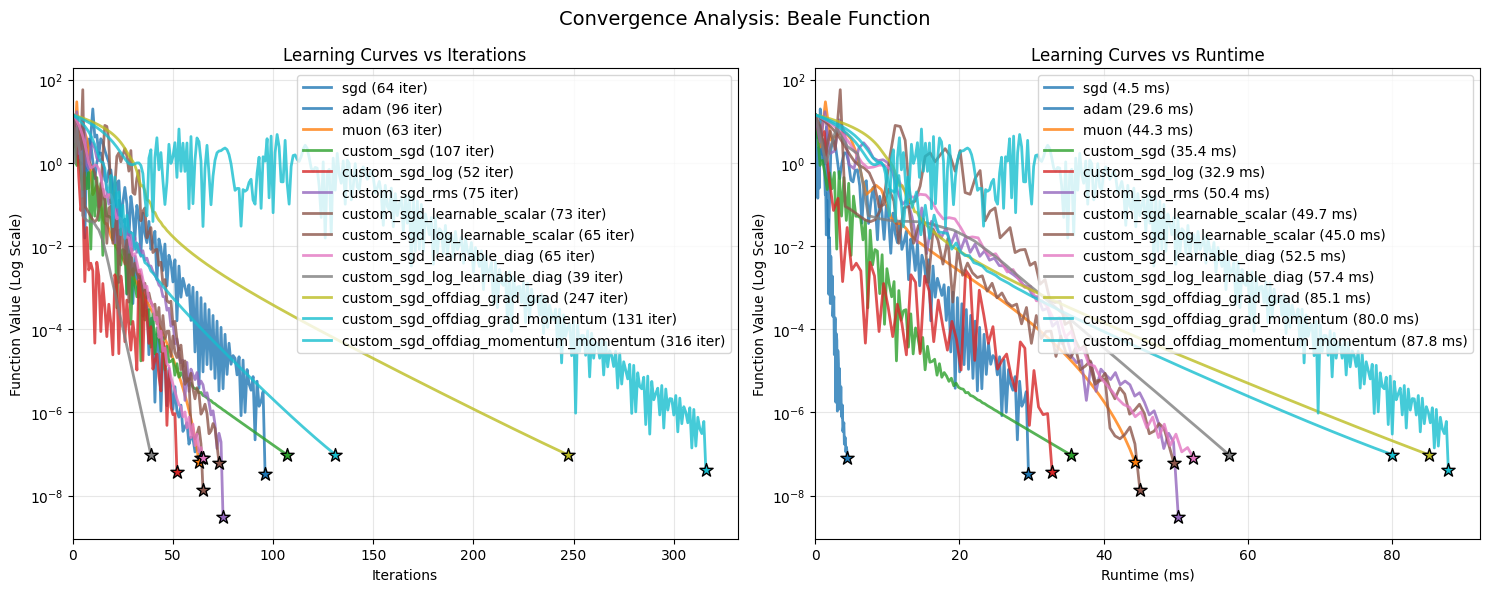
\includegraphics[width=\textwidth]{../images/Beale_116da11.png}
    \end{minipage}
    \begin{minipage}{0.70\textwidth}
        \centering
        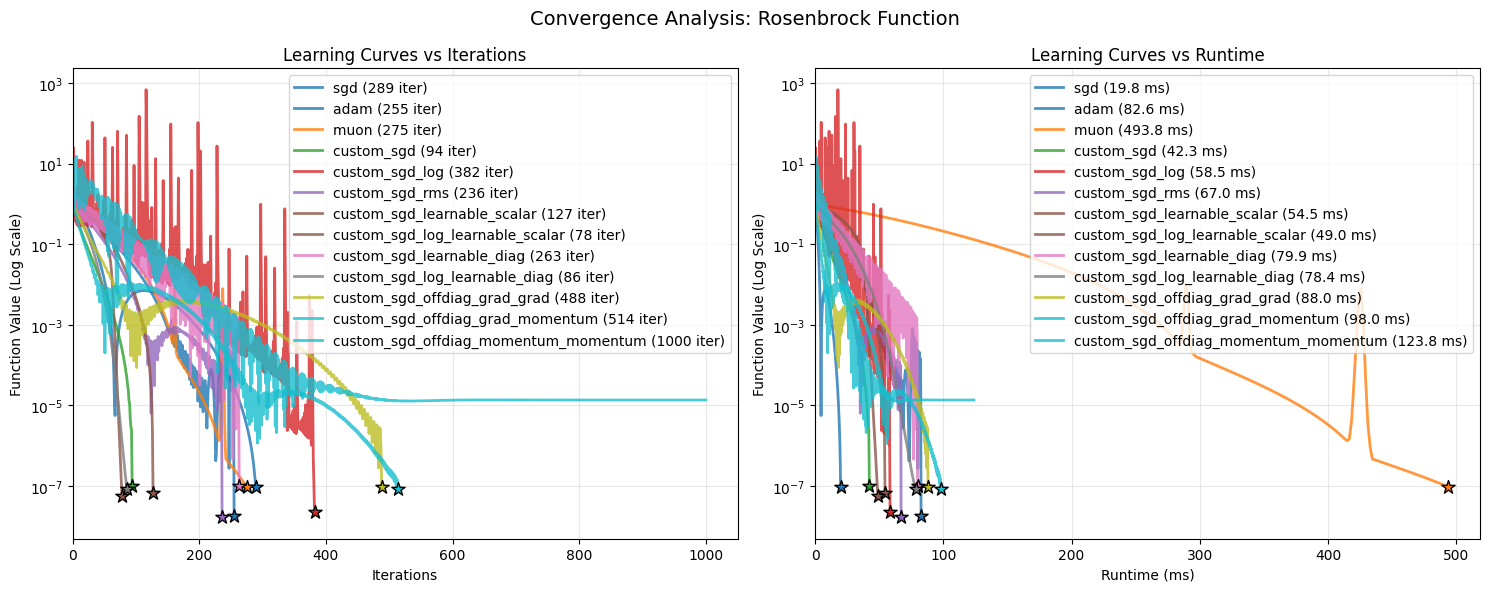
\includegraphics[width=\textwidth]{../images/Rosenbrock_116da11.png}
    \end{minipage}
    \begin{minipage}{0.70\textwidth}
        \centering
        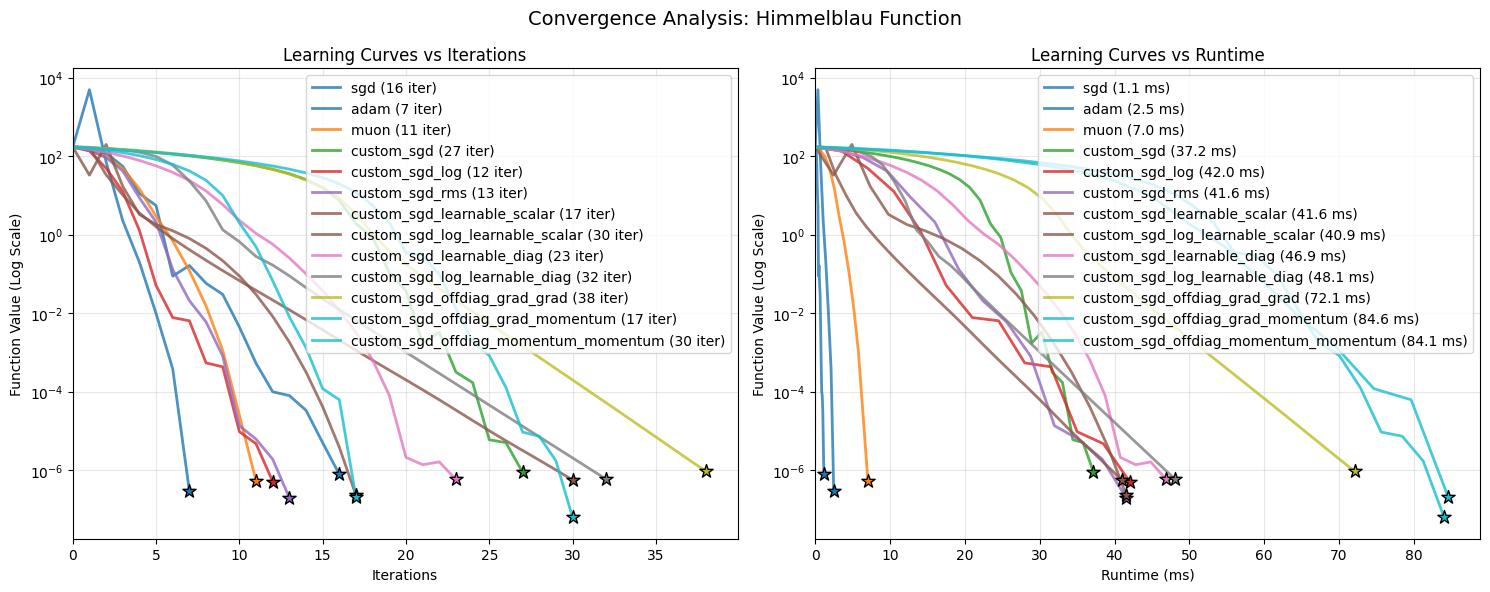
\includegraphics[width=\textwidth]{../images/Himmelblau_116da11.png}
    \end{minipage}
    \begin{minipage}{0.70\textwidth}
        \centering
        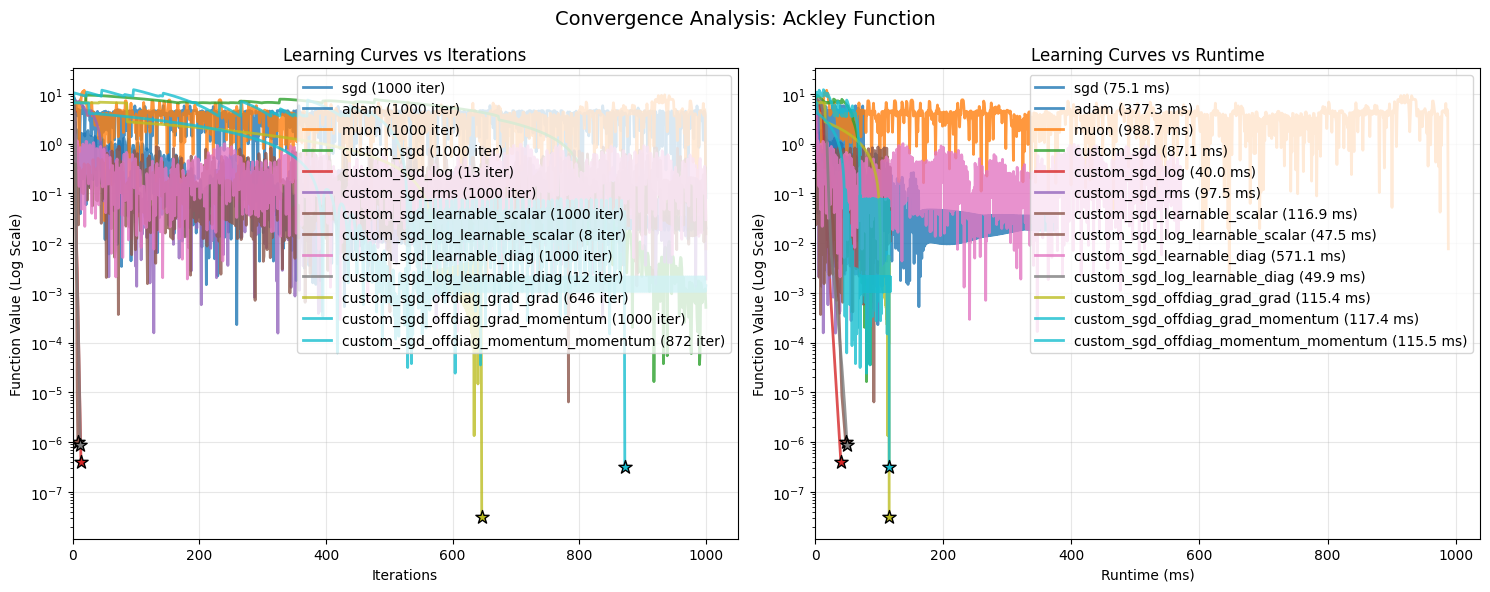
\includegraphics[width=\textwidth]{../images/Ackley_116da11.png}
    \end{minipage}
    \begin{minipage}{0.70\textwidth}
        \centering
        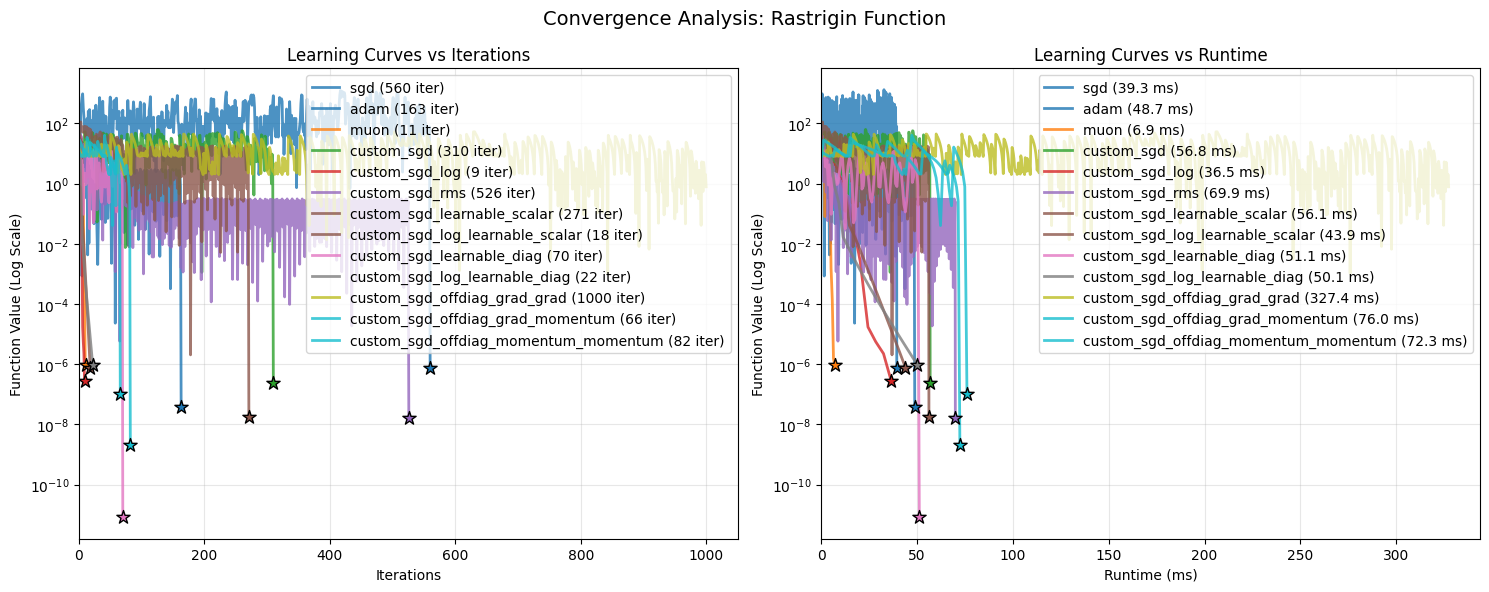
\includegraphics[width=\textwidth]{../images/Rastrigin_116da11.png}
    \end{minipage}
    \caption{
        Small-example benchmark results for all optimiser variants.
        Each plot shows the best hyperparameter configuration found by the sweep.
        \textit{(Fixed and off-diagonal sweeps are complete for small examples.)}
    }
\end{figure}


%%%%%%%%%%%%%%%%%%%%%%%%%%%%%%%%%%%%%%%%%%%%%%%%%%%%%%%%%%%%%
%%%%%%%%%%%%%%%%%%%%%%%%%%%%%%%%%%%%%%%%%%%%%%%%%%%%%%%%%%%%%
\begin{appendices}
\section{Repository Structure}\label{app:repo}
%%%%%%%%%%%%%%%%%%%%%%%%%%%%%%%%%%%%%%%%%%%%%%%%%%%%%%%%%%%%%
%%%%%%%%%%%%%%%%%%%%%%%%%%%%%%%%%%%%%%%%%%%%%%%%%%%%%%%%%%%%%

\subsection{Directory Layout}
\begin{center}
\small
\begin{tabular}{@{}lp{8cm}@{}}
    \toprule
    \textbf{Directory} & \textbf{Contents} \\
    \midrule
    \texttt{optimisers/}  & JAX and PyTorch optimiser implementations and equivalence checks \\
    \texttt{parameters/}  & Hyperparameter sweep scripts and shared training utilities \\
    \texttt{analysis/}    & Jupyter notebooks for loading and visualising sweep results \\
    \texttt{documents/}   & This document and supplementary notebooks \\
    \texttt{images/}      & Figures used in \cite{harvey2025} and this document \\
    \texttt{results/}     & Local sweep results (JSON, gitignored) \\
    \texttt{data/}        & Local data files (gitignored) \\
    \bottomrule
\end{tabular}
\end{center}

\subsection{Running Sweeps}
Hyperparameter sweeps are driven by scripts in \texttt{parameters/} and support two backends:
\textbf{local} (Optuna + JSON files, no account required) and \textbf{WandB} (cloud logging).

\begin{center}
\small
\begin{tabular}{lll}
    \toprule
    \textbf{Script} & \textbf{Task} & \textbf{Model} \\
    \midrule
    \texttt{sweep\_mnist\_mlp.py}       & MNIST classification        & MLP (64 hidden) \\
    \texttt{sweep\_cifar10\_resnet18.py} & CIFAR-10 classification     & ResNet-18 \\
    \texttt{sweep\_regression.py}        & Synthetic regression        & MLP \\
    \texttt{sweep\_shake.py}             & Shakespeare language model  & MiniGPT \\
    \texttt{sweep\_small\_examples.py}   & 2D test functions           & n/a \\
    \bottomrule
\end{tabular}
\end{center}

All scripts share a common CLI:
\begin{itemize}
    \item \texttt{--optimiser}: optimiser name (see below).
    \item \texttt{--num\_runs}: number of Optuna trials (default: 50).
    \item \texttt{--backend}: \texttt{local} or \texttt{wandb} (default: \texttt{wandb}).
    \item \texttt{--index}: run index for organising multiple runs of the same sweep.
\end{itemize}
\begin{sloppypar}
Results are written to \path{results/<task>/<optimiser>/run_<index>/<run_id>.json},
each containing the full training history, final summary metrics, and the hyperparameter config used.
\end{sloppypar}

\subsection{Available Optimisers}
\begin{center}
\footnotesize
\begin{tabular}{@{}lp{6cm}@{}}
    \toprule
    \textbf{Sweep name} & \textbf{Description} \\
    \midrule
    \texttt{adam}, \texttt{adamw}, \texttt{sgd}, \texttt{muon} & Baselines \\
    \texttt{sgd\_metric}, \texttt{sgd\_log\_metric}, \texttt{sgd\_rms} & Fixed diagonal metric \\
    \texttt{sgd\_learn\_scalar}, \texttt{sgd\_learn\_scalar\_log} & Learnable scalar metric \\
    \texttt{sgd\_learn\_diag}, \texttt{sgd\_learn\_diag\_log} & Learnable diagonal metric \\
    \texttt{sgd\_offdiag\_\{a\}\_\{b\}} & Off-diagonal metric ($\{0,l,m,\theta\}^2$ pairs, excluding $0\_0$) \\
    \bottomrule
\end{tabular}
\end{center}
The full optimiser registry is \href{https://github.com/Noah-Everett/Induced-Metric-Optimiser/blob/main/parameters/optimizer_registry.py}{\texttt{parameters/optimizer\_registry.py}}.

\subsection{Analysis Notebooks}
\begin{center}
\small
\begin{tabular}{@{}lp{6cm}@{}}
    \toprule
    \textbf{Notebook} & \textbf{Task} \\
    \midrule
    \texttt{analysis/small\_examples.ipynb}   & 2D test functions (Beale, Rosenbrock, etc.) \\
    \texttt{analysis/mnist\_analysis.ipynb}   & MNIST MLP \\
    \texttt{analysis/cifar\_analysis.ipynb}   & CIFAR-10 ResNet-18 \\
    \texttt{analysis/regression\_analysis.ipynb} & Synthetic regression \\
    \texttt{analysis/shake\_analysis.ipynb}   & Shakespeare language modelling \\
    \bottomrule
\end{tabular}
\end{center}
Each notebook supports both backends.
Configure \texttt{BACKEND}, \texttt{TASK\_TAG}, and \texttt{OPTIMIZERS} in the second cell.
Outputs include training curves, 2D histograms of best metric vs.\ epoch,
time-to-best analysis, and best-hyperparameter tables (also saved as CSV to \texttt{analysis/}).

\end{appendices}


\begin{thebibliography}{1}
\bibitem{harvey2025}
T.~R.~Harvey,
``The Optimiser Hidden in Plain Sight: Training with the Loss Landscape's Induced Metric,''
\emph{arXiv preprint arXiv:2509.03594}, 2025.
\end{thebibliography}

\end{document}
